\newcommand{\DoNotLoadEpstopdf}{} % No EPS conversion or shell execution is needed.
\documentclass[11pt,letterpaper]{article}
\usepackage[T1]{fontenc}
\usepackage[utf8]{inputenc}
\usepackage[margin=.87in,top=.83in,bottom=.87in,headheight=23pt,headsep=.22in]{geometry}
\usepackage{amsmath,amsthm,mathtools}
\usepackage{newpxtext,newpxmath}
\usepackage{microtype}
\usepackage{booktabs,tabularx,array,longtable,multirow}
\usepackage{graphicx,xcolor,tikz,pgfplots}
\usetikzlibrary{arrows.meta,positioning,calc,fit,backgrounds,decorations.pathmorphing}
\pgfplotsset{compat=1.18}
\usepackage[most]{tcolorbox}
\usepackage{enumitem,needspace,fancyhdr,titlesec,caption,float,placeins}
\usepackage{listings,xurl,upquote}
\usepackage[numbers,sort&compress]{natbib}
\usepackage[unicode,bookmarksnumbered]{hyperref}
\usepackage{bookmark}
\definecolor{Ink}{HTML}{221A2D}
\definecolor{Violet}{HTML}{3E244B}
\definecolor{Gold}{HTML}{A87724}
\definecolor{LightGold}{HTML}{E4BF73}
\definecolor{Ivory}{HTML}{FBF8F0}
\definecolor{Muted}{HTML}{635C69}
\definecolor{Rule}{HTML}{D9CFBE}
\definecolor{Pale}{HTML}{F4F0F6}
\hypersetup{pdftitle={ALPHA GENESIS FLYWHEEL OMEGA: Riding the Exponential},pdfauthor={Vincent Boucher},pdfsubject={Transformational Intelligence: frontier-coupled autonomous discovery, commercial compounding, and productive expansion},pdfkeywords={ALPHA GENESIS, SUCCESSOR OMEGA, transformational intelligence, autonomous discovery, frontier replay, scientific instruments, economic invention},colorlinks=true,linkcolor=Violet,citecolor=Violet,urlcolor=Violet}
\pagestyle{fancy}\fancyhf{}
\fancyhead[L]{\footnotesize\sffamily\color{Muted}ALPHA GENESIS FLYWHEEL $\Omega$}
\fancyhead[R]{\footnotesize\sffamily\color{Muted}Boucher \;|\; Research release 1.1}
\fancyfoot[L]{\scriptsize\sffamily\color{Muted}TRANSFORMATIONAL INTELLIGENCE $\infty$}
\fancyfoot[R]{\small\color{Gold}\thepage}
\renewcommand{\headrulewidth}{.35pt}
\renewcommand{\headrule}{\hbox to\headwidth{\color{Rule}\leaders\hrule height \headrulewidth\hfill}}
\setlength{\parindent}{0pt}
\setlength{\parskip}{.48em plus .08em minus .05em}
\setlength{\emergencystretch}{2.5em}
\linespread{1.045}
\raggedbottom
\widowpenalty=10000
\clubpenalty=10000
\titleformat{\section}{\Large\bfseries\color{Violet}}{\color{Gold}\thesection}{.7em}{}
\titleformat{\subsection}{\large\bfseries\color{Ink}}{\thesubsection}{.7em}{}
\titleformat{\subsubsection}{\normalsize\bfseries\color{Ink}}{\thesubsubsection}{.7em}{}
\titlespacing*{\section}{0pt}{2.1ex plus .6ex minus .2ex}{.8ex}
\titlespacing*{\subsection}{0pt}{1.5ex plus .4ex minus .2ex}{.4ex}
\captionsetup{font=small,labelfont={bf,color=Violet},textfont={color=Muted},skip=7pt}
\setlist{leftmargin=1.4em,itemsep=.15em,topsep=.2em,parsep=0pt}
\renewcommand{\arraystretch}{1.16}
\newcolumntype{Y}{>{\raggedright\arraybackslash}X}
\newcolumntype{P}[1]{>{\raggedright\arraybackslash}p{#1}}
\newcommand{\E}{\mathbb{E}}
\newcommand{\Prob}{\mathbb{P}}
\newcommand{\I}{\mathcal{I}}
\newcommand{\R}{\mathcal{R}}
\newcommand{\Hh}{\mathcal{H}}
\newcommand{\GG}{\mathcal{G}}
\newcommand{\ind}{\mathbf{1}}
\newcommand{\OmegaName}{SUCCESSOR $\Omega$}
\newcommand{\Genesis}{GENESIS}
\DeclareMathOperator*{\argmax}{arg\,max}
\DeclareMathOperator*{\argmin}{arg\,min}
\DeclareMathOperator{\rank}{rank}
\newtheorem{definition}{Definition}[section]
\newtheorem{proposition}{Proposition}[section]
\theoremstyle{remark}\newtheorem{remark}{Remark}[section]
\newtcolorbox{thesisbox}{enhanced,breakable,colback=Ivory,colframe=Gold,boxrule=.5pt,arc=1.5mm,left=12pt,right=12pt,top=9pt,bottom=9pt,before skip=10pt,after skip=10pt}
\newtcolorbox{statusbox}{enhanced,breakable,colback=Pale,colframe=Violet,boxrule=0pt,borderline west={2.5pt}{0pt}{Violet},arc=0mm,left=11pt,right=11pt,top=8pt,bottom=8pt,before skip=9pt,after skip=9pt}
\newcommand{\smallhead}[1]{\par\smallskip{\sffamily\bfseries\color{Gold}#1}\par\smallskip}
\lstset{upquote=true,basicstyle=\small\ttfamily,breaklines=true,columns=fullflexible,keepspaces=true,showstringspaces=false,frame=single,rulecolor=\color{Rule},backgroundcolor=\color{Ivory},xleftmargin=5pt,xrightmargin=5pt,framesep=7pt}
\setcounter{tocdepth}{1}
\renewcommand{\topfraction}{.85}
\renewcommand{\textfraction}{.08}
\renewcommand{\floatpagefraction}{.8}
\begin{document}

% ---------- COVER ----------
\begin{titlepage}
\thispagestyle{empty}

\begin{tikzpicture}[remember picture,overlay]
\fill[Ink] (current page.south west) rectangle (current page.north east);
\fill[Violet,opacity=.4] ([yshift=2.2in]current page.south west) rectangle ([yshift=-3.4in]current page.north east);
\draw[LightGold,line width=.8pt] ([xshift=.35in,yshift=.35in]current page.south west) rectangle ([xshift=-.35in,yshift=-.35in]current page.north east);
\draw[LightGold,opacity=.35,line width=.35pt] ([xshift=.43in,yshift=.43in]current page.south west) rectangle ([xshift=-.43in,yshift=-.43in]current page.north east);
\node[anchor=north west,text=LightGold,font=\sffamily\small] at ([xshift=.75in,yshift=-.7in]current page.north west) {MONTREAL.AI\quad /\quad QUEBEC.AI};
\node[anchor=north east,text=LightGold,font=\sffamily\small] at ([xshift=-.75in,yshift=-.7in]current page.north east) {RESEARCH RELEASE 1.1};
\node[anchor=north,text=Ivory,font=\fontsize{31}{35}\selectfont] at ([yshift=-1.35in]current page.north) {ALPHA};
\node[anchor=north,text=LightGold,font=\fontsize{62}{67}\selectfont\bfseries] at ([yshift=-1.95in]current page.north) {GENESIS};
\node[anchor=north,text=Ivory,font=\fontsize{27}{32}\selectfont] at ([yshift=-2.94in]current page.north) {FLYWHEEL $\Omega$};
\node[anchor=north,align=center,text=Ivory,text width=6.7in,font=\fontsize{16}{21}\selectfont] at ([yshift=-3.65in]current page.north) {Turn the next advance in AI into your next ability\\to autonomously discover at scale.};
\coordinate (O) at ([yshift=-6.4in]current page.north);
\foreach \r in {1.00,1.12,1.47,1.55}{\draw[LightGold,opacity=.6,line width=.65pt] (O) circle (\r in);}
\foreach \ang in {0,60,120}{\draw[LightGold,opacity=.4,rotate around={\ang:(O)}] (O) ellipse (2.25in and .63in);}
\foreach \ang in {0,30,...,330}{\draw[LightGold,opacity=.25] (O) -- ($(O)+(\ang:1.47in)$);}
\foreach \ang in {25,145,265}{\fill[LightGold] ($(O)+(\ang:1.47in)$) circle (3.5pt);\draw[LightGold,opacity=.4] ($(O)+(\ang:1.47in)$) circle (7pt);}
\node[text=LightGold,font=\fontsize{83}{88}\selectfont] at (O) {$\Omega$};
\node[text=Ivory,font=\sffamily\small,fill=Ink,inner sep=5pt] at ($(O)+(90:1.55in)$) {NEW INTELLIGENCE};
\node[text=Ivory,font=\sffamily\small,fill=Ink,inner sep=5pt] at ($(O)+(210:1.92in)$) {VERIFIED MEANS};
\node[text=Ivory,font=\sffamily\small,fill=Ink,inner sep=5pt] at ($(O)+(330:1.92in)$) {STRONGER SUCCESSORS};
\node[anchor=north,text=LightGold,font=\sffamily\bfseries\large] at ([yshift=-8.55in]current page.north) {RIDING THE EXPONENTIAL};
\node[anchor=north,text=Ivory,align=center,text width=6.5in,font=\large] at ([yshift=-8.95in]current page.north) {Invent the means. Expand what becomes possible.\\Compound the ability to discover.};
\node[anchor=south west,text=Ivory,align=left,font=\normalsize] at ([xshift=.75in,yshift=.83in]current page.south west) {\textbf{Vincent Boucher}\\President of MONTREAL.AI};
\node[anchor=south east,text=LightGold,align=right,font=\small] at ([xshift=-.75in,yshift=.83in]current page.south east) {TRANSFORMATIONAL INTELLIGENCE $\infty$\\4 November 2026};
\end{tikzpicture}
\null
\end{titlepage}
\setcounter{page}{1}

% ---------- ABSTRACT ----------
\begin{center}
{\small\sffamily\color{Gold}THE ADVANTAGE WORTH BUILDING}\par\vspace{.3em}
{\LARGE\bfseries\color{Violet}ALPHA GENESIS FLYWHEEL $\Omega$}\par\vspace{.4em}
{\large Riding the exponential: from frontier intelligence\\to compounding discovery and productive power}\par\vspace{.8em}
{Vincent Boucher\quad $\cdot$\quad MONTREAL.AI / QUEBEC.AI}\par
{\small Montr\'eal, Qu\'ebec, Canada\quad $\cdot$\quad 4 November 2026}
\end{center}
\smallhead{ABSTRACT}
Frontier AI advances create opportunities, but access to stronger models does not by itself create an enduring institution, a profitable business, or a new scientific capability. We propose \emph{ALPHA GENESIS FLYWHEEL $\Omega$}: a customer-owned discovery foundry that converts newly accessible intelligence into executable means, qualifies their usefulness, and tests whether retained means improve fresh successor construction. Building on \emph{Transformational Intelligence}, the object of invention includes the problem formulation, experimental instruments, representations, production processes, and voluntary economic arrangements---not merely answers inside a fixed workflow. The architecture connects opportunity selection (Alpha), development environments (Gym), protected comparative qualification, and institutional continuity (SUCCESSOR $\Omega$). Its distinctive operating proposal is \emph{Frontier Replay}: relevant advances reopen specific blocked opportunities, while new candidates face fresh evidence rather than inherit old approval. We distinguish external model progress, inherited capabilities, improved discovery procedures, commercial compounding, and physical expansion. A conditional adoption-lag analysis explains why faster qualified conversion can matter even when access to intelligence is shared. An executable companion supplies an exact observation-construction witness, independently implemented replay controls, adversarial access and relevance cases, and cash-flow counterexamples; capable conventional methods tie the supplied constructions. These results establish the stated calculations, not autonomous scientific superiority. We specify a self-service product, public-component engineering path, rigorous campaign-level experiments, and a commercial mechanism that can finance further productive capacity. The long horizon is a chain from better instruments to energy, manufacturing, and increasingly capable space infrastructure. Each transition is a construction problem with its own evidence, economics, and physical limits.

\begin{statusbox}
\textbf{Research status.} This release delivers a research synthesis, an implementable product specification, analytic propositions, and executed finite-model and publication-integrity checks. It does not report a deployed GENESIS product, new physical measurements, paying customers, or a completed open-ended self-improvement system. Source-reported historical results remain separate from this edition's computations.
\end{statusbox}
\textbf{Keywords:} transformational intelligence; autonomous discovery; frontier adaptation; generative capability; scientific instruments; economic invention; institutional memory.

\clearpage
\smallhead{THE PAPER AT A GLANCE}
\begin{thesisbox}
\Large\bfseries An AI advance is a new input.\\A verified capability is a new asset.\\A better way to construct successors is the deeper advantage.
\end{thesisbox}
\textbf{The product.} A local-first, self-service discovery application. A user supplies a consequential objective, authorized evidence, available equipment or compute, and a resource budget. The application constructs competing means, executes discriminating experiments, exports usable artifacts, and retains only the scope its evidence supports.

\textbf{The inventive engine.} Diagnose what prevents the outcome. Construct a missing means, change the representation or arrangement, or eliminate an unnecessary dependency. The means of invention are themselves revisable; the purpose and the basis for accepting claims are not silently rewritten.

\textbf{The frontier connection.} A release is relevant only when it changes an actual construction opportunity. Verify access, revisit the recorded obstacle, build a challenger, test it on fresh work, and adopt only the supported improvement.

\textbf{The commercial connection.} Deliver a buyer-valued outcome, collect payment, cover complete costs and obligations, and direct genuinely available resources to the most valuable next capability or growth channel. Ordinary profitable delivery need not wait for recursive discovery.

\textbf{The long horizon.} Use qualified means to construct better observation, experimentation, production, energy, and infrastructure. The chain is ambitious precisely because its physical and commercial transitions are explicit, rather than assumed.

\begin{center}
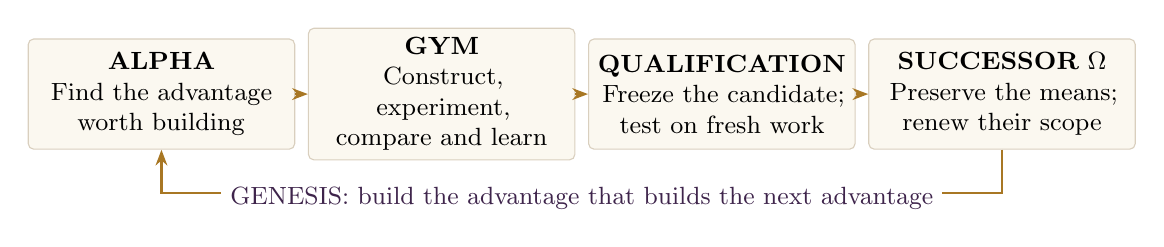
\begin{tikzpicture}[node distance=.16cm, every node/.style={align=center,font=\small}, box/.style={draw=Rule,fill=Ivory,rounded corners=2pt,text width=3.15cm,minimum height=1.4cm},arr/.style={-{Stealth[length=2mm]},thick,Gold}]
\node[box] (a) {\textbf{ALPHA}\\Find the advantage\\worth building};
\node[box,right=of a] (b) {\textbf{GYM}\\Construct, experiment,\\compare and learn};
\node[box,right=of b] (c) {\textbf{QUALIFICATION}\\Freeze the candidate;\\test on fresh work};
\node[box,right=of c] (d) {\textbf{SUCCESSOR $\Omega$}\\Preserve the means;\\renew their scope};
\draw[arr] (a)--(b);\draw[arr] (b)--(c);\draw[arr] (c)--(d);
\draw[arr] (d.south) -- ++(0,-.55) -| (a.south);
\node[fill=white,text=Violet] at ($(b.south)!.5!(c.south)+(0,-.55)$) {GENESIS: build the advantage that builds the next advantage};
\end{tikzpicture}
\end{center}
\vspace{.2em}
\textbf{Read by purpose.} The strategic argument begins in Sections~\ref{sec:thesis}--\ref{sec:transform}. The operating and product design is in Sections~\ref{sec:institution}--\ref{sec:product}. The experiments and commercial logic are in Sections~\ref{sec:evaluation}--\ref{sec:commerce}. The physical horizon, decisive programme, and release contract (Section~\ref{sec:release}) close the paper. Appendix~\ref{app:reproduce} explains how to reproduce the calculations.
\clearpage
\tableofcontents

\clearpage
\section{The advantage worth building}
\label{sec:thesis}
The central entrepreneurial question is not which model is most impressive this week. It is which valuable activity has become achievable, what must be constructed to realize it, and what the resulting capability makes possible next. A model release is an opportunity to investigate. A production-ready instrument, a usable scientific method, or a complete commercial arrangement is a different achievement.

We propose an enterprise that continually works across that difference. Its products are useful capabilities. Its deeper asset is an increasingly effective ability to construct them. Its institutional memory preserves methods, evidence, skills, limitations, and operating experience across changes in models. Its commercial operation supplies resources and consequential problems without requiring every profitable delivery to be a scientific breakthrough.

\begin{thesisbox}
\textbf{The founding hypothesis.} An institution that repeatedly converts relevant AI advances into qualified productive means---and tests how those means improve subsequent construction---can acquire an advantage that is not reducible to access to the underlying model.
\end{thesisbox}

This is a hypothesis about a working system, not a prediction that intelligence or profit grows indefinitely. The author-supplied research makes the critical distinction: a working invention, a useful inheritance, and an improved method of invention are separate claims \citep{notes30,notes29}. A library can grow while becoming less useful. A newer model can improve outputs while the institution contributes nothing. A commercially successful operation can expand with a fixed model. Each possibility must remain visible.

\subsection{Alpha is relative to a mission and a complete alternative}
For a declared task population, horizon, and cost basis, let $J_{\I}(s)$ denote mission value delivered by system $s$, after the costs included in that mission's value model. Hard requirements remain constraints rather than tradable score bonuses. Given a nonempty, disclosed set $\mathcal B$ of capable feasible alternatives, define
\begin{equation}
\alpha_{\I}(s;\mathcal B)=J_{\I}(s)-\max_{b\in\mathcal B}J_{\I}(b).
\label{eq:alpha}
\end{equation}
The baseline set includes the incumbent and the strongest credible complete routes actually available for comparison. It can contain a specialist, an unrestricted frontier agent, conventional engineering, procurement, customer self-service, and non-entry. Equation~\eqref{eq:alpha} is a definition, not an estimator of an unknown global optimum. Where values are multidimensional, report the trade-off frontier instead of inventing a convenient exchange rate between quality, risk, time, and money.

A useful local improvement may beat the incumbent yet lose to another available method. A construction may enable a previously inaccessible installed capability yet be discovered equally well by a conventional engineer. A business may profit without either kind of invention superiority. These are different, legitimate outcomes; none should be relabeled to manufacture the others.

\subsection{The ambition is larger than a task catalogue}
The consequential search space includes new observations, scientific representations, experimental procedures, algorithms, interfaces, manufacturing processes, and economic arrangements. It also includes changes that make a supposedly necessary subproblem disappear. If a recurring measurement is costly, the best invention might be a better instrument, a selective-use policy, or a production change that eliminates the relevant uncertainty. The desired outcome, not the inherited method, determines which route is admissible \citep{transform,notes29}.

This is why electrical tomography is a candidate test domain rather than GENESIS's permanent identity. It offers concrete observations, physical uncertainty, and public engineering tools. It does not establish that an electrical scanner is the strongest commercial opportunity. The product is the construction of useful research capabilities; the first domain must earn its role through evidence.

\section{What the frontier now makes worth attempting}
\label{sec:frontier}
The evidence cutoff for this edition is \textbf{4 November 2026}. Table~\ref{tab:frontier} separates recent demonstrations, actual access conditions, and the decisions they motivate. An announcement date is not the date a task first became possible. An internal result is not an available production dependency. A scientific preprint is not industrial qualification.

\begin{table}[htbp]
\small
\caption{A dated frontier snapshot. Provider reports support the described capabilities, not GENESIS's proposed integrated performance.}
\label{tab:frontier}
\begin{tabularx}{\linewidth}{P{2.1cm}YY}
\toprule
\textbf{Date / source}&\textbf{Verified development}&\textbf{Consequence for GENESIS}\\\midrule
3 Nov 2026\newline OpenAI \citep{engineering}&Astra-assisted enclosure, PCB, software, and prototype workflow; manufacturing review remained necessary. A stronger engineering model is internal.&Construct connected engineering packages. Test tolerances, interfaces, and manufacturability rather than assuming them.\\
3 Nov 2026\newline DeepMind \citep{chemistry}&Antigravity cheminformatics skills connect scientific reasoning with deterministic tools; proposed compounds still require experiments.&Make a scientific skill executable. Do not confuse computational proposals with measured properties.\\
3 Nov update\newline Google Research \citep{era}&Computational Discovery, built with ERA and AlphaEvolve, adds an MCP integration route for approved users.&Scientific orchestration is a capable alternative, not an untouched market. Restricted access cannot be assumed.\\
1 Nov revision\newline Hyperagents \citep{hyperagents}&The revised preprint studies editable task and meta-agent code. Its title page is dated 3 Nov; the arXiv revision is dated 1 Nov.&Treat the improvement procedure itself as a candidate object. Compare against this research, not only fixed workflows.\\
26 / 30 Oct\newline OpenAI \citep{modelnotes}&GPT-6.1 Terra rollout includes Work and Codex. GPT-6 Rosalind Research requires specific approval.&Verify the user's accessible model and tools. Version names alone do not establish a usable capability.\\
21 Oct 2026\newline OpenAI \citep{biology}&Thousands of agents analyzed existing biological data, generating research leads for further investigation.&Parallelize complete investigations where useful; candidate explanations are not validated treatments.\\
Current collection\newline OpenAI \citep{openaimath}&Public mathematical manuscripts and proof artifacts have different verification stages; the generating model is internal.&Investigate applicable results and proof dependencies. A theorem, its formalization, and a usable algorithm are distinct assets.\\\bottomrule
\end{tabularx}
\end{table}

The physical-engineering report is especially relevant because it connects mechanical, electrical, and software work rather than presenting isolated artifacts. Its remaining manufacturing corrections identify useful engineering targets. The scientific-skills release supplies a complementary pattern: model reasoning coordinates domain tools, while those tools perform explicit calculations. Neither report demonstrates an autonomous instrument foundry. Together they justify testing a more integrated construction process \citep{engineering,chemistry}.

The mathematics repository reports 721 manuscripts in 373 families, with roughly 42\% of top-line results formalized at the inspected snapshot. It describes the collection as raw research material and acknowledges that unformalized results may contain issues \citep{openaimath}. GENESIS should preserve the exact theorem statement, assumptions, formal dependencies, and application bridge before building on any result. Mathematical importance alone does not establish a practical runtime advantage, a finite-noise reconstruction method, or commercial demand.

\subsection{Research precedents raise the bar}
AlphaEvolve combines generated code, evolutionary search, and evaluation in scientific and computational problems \citep{alphaevolve}. Automated Design of Agentic Systems searches executable agent designs \citep{adas}. The Darwin G\"odel Machine explores empirically evaluated self-modifications \citep{dgm}. Hyperagents makes the meta-level modification procedure editable and reports transfer in its studied settings \citep{hyperagents}. These are direct comparators and sources of mechanisms, not proof that our integrated economic and physical programme already exists.

DreamCoder illustrates learning reusable abstractions alongside program search, while POET illustrates the joint development of environments and solutions with transfer \citep{dreamcoder,poet}. The contribution proposed here is not ownership of those ideas. It is their disciplined connection to purpose-preserving formulation change, frontier-triggered opportunity reopening, independently evaluated successor benefit, and complete productive economics.

\section{Transformational intelligence: invent the means, or remove the need}
\label{sec:transform}
The foundational manuscript separates \emph{purpose}, \emph{formulation}, and \emph{evaluation} \citep{transform}. We retain that distinction. An intent charter is
\begin{equation}
\I=(\mathcal D,U,\mathcal C,\mathcal A,\mathbf b),
\end{equation}
where $\mathcal D$ describes initial task conditions, $U$ the authorized outcome, $\mathcal C$ material requirements, $\mathcal A$ permitted actions, and $\mathbf b$ resource constraints. A formulation
\begin{equation}
F=(R,K,Q,\Pi,\nu)
\end{equation}
specifies representations, assumptions, information procedures, executable policy language, and intermediate objectives. An evaluation instrument $E$ measures the relationship between actual behavior and the authorized outcome. None is automatically a perfect proxy for another.

A proposed transformation has the inherited form
\begin{equation}
T=(F',C_T,L_T,W_T),
\label{eq:transform}
\end{equation}
where $C_T$ constructs the means required by the new formulation, $L_T$ realizes it in the original setting, and $W_T$ records the changed restriction, the outcome bridge, and a potential falsifier. A paragraph about a new way to think is not sufficient: the changed method must have executable meaning.

\subsection{Four constructive responses to an obstacle}
A verified failure can justify repairing a solver within its existing setup. It can also justify acquiring information, constructing a different operation, or removing a dependency. GENESIS must investigate these alternatives rather than default to more agents. The distinction is particularly important when a missing means is only required by the current strategy.

\begin{table}[htbp]
\caption{The object of invention can be the conditions of useful work. These are starting examples, not a fixed grammar.}
\begin{tabularx}{\linewidth}{P{3.1cm}YY}
\toprule
\textbf{Observed obstacle}&\textbf{Possible construction}&\textbf{What must be tested}\\\midrule
Two explanations fit the same observations&New excitation, reference experiment, or sensor arrangement&Does newly acquired evidence distinguish the decision-relevant states?\\
A representation hides a useful relationship&Invariant, symbolic language, or causal abstraction&Does it preserve required distinctions and reduce complete construction cost?\\
Verification reconstructs lost evidence&Evidence-preserving production plus a compatible checker&Are accepted outcomes better or cheaper after both components are counted?\\
A process cannot finance its first delivery&Staging, shared construction, or different payment terms&Do real participants prefer the arrangement, and does cash remain sufficient?\\
Search repeatedly misses the useful route&A revised generator, retrieval method, or discovery policy&Does it produce better capabilities in fresh complete campaigns?\\\bottomrule
\end{tabularx}
\end{table}

The source discussions supply two complementary generators: structural transfer and adversarial discovery \citep{notes30,notes29,notes18}. Structural transfer maps relationships, assumptions, and mechanisms across domains rather than matching vocabulary. Adversarial discovery seeks a consequential, independently checkable failure rather than agreement among fluent critics. Where an analogy breaks, the response can be rejection, construction of the missing correspondence, or a reformulation that avoids needing it.

Criticism is itself fallible. A failed critic may require a better experiment or representation, but adding critics does not create independent evidence. The original source must remain accessible for source-based claims; physical claims require suitable physical observations. An objection is a candidate finding until checked \citep{notes18,critic}.

\subsection{The retained asset has three possible depths}
A campaign can leave a working instrument; an applicability model describing where it works; and a generative procedure for constructing related instruments. Only the first may initially be supported. The latter two require additional tests. A reusable explanation is not automatically a reusable constructor, and a constructor is not automatically an improved method for discovering constructors.

The institution records enabling relationships as hypotheses until interventions support them. A useful relationship says: acquiring capability $a$ changed the feasibility, quality, or complete cost of constructing $b$, under specified conditions. It does not say merely that $a$ happened before $b$. Several parents may be jointly necessary, so a capability graph must support hyperedges rather than force every effect into a single-parent story.

\begin{thesisbox}
\textbf{The unit that compounds is not the answer. It is a supported change in what the next campaign can discover, construct, verify, or economically deliver.}
\end{thesisbox}

\section{The institution behind the flywheel}
\label{sec:institution}
The supplied visual references express a four-stage journey: \emph{Alpha $\rightarrow$ Gym $\rightarrow$ Specialist ASI $\rightarrow$ SUCCESSOR $\Omega$}. We preserve its organization while making each stage operational. The images are conceptual communication artifacts, not evidence that the depicted capabilities are implemented.

\textbf{Alpha selects the advantage.} It identifies the beneficiary, consequential outcome, strongest complete alternative, unresolved constraint, and smallest decisive construction. The opportunity is assessed after construction, checking, adoption, maintenance, human effort actually required, and competitive response.

\textbf{Gym develops the capability.} It turns authorized evidence, tools, constraints, and experimental history into executable environments. Candidate constructors may change workflows, abstractions, experiments, and internal organization. Development feedback improves a candidate; it does not certify it. Simulation guides physical experiments rather than replaces them.

\textbf{Qualification makes the claim earn its scope.} Freeze a candidate, its permitted adaptation policy, comparators, measurement, and accounting. Evaluate it on fresh work. The source visuals use \emph{Specialist ASI} as a mission-specific designation. In this paper it is project terminology, not a recognized certification or evidence of general superintelligence. The scientific claim remains the measured advantage, task population, resources, and uncertainty. A small benchmark win alone does not warrant the designation.

\textbf{SUCCESSOR $\Omega$ preserves continuity.} Retain executable methods, relevant evidence, skills, lessons, and operating history. Models can be replaced without erasing the mission. But ownership of records is not ownership of a provider's model weights, and portability does not eliminate dependence on model access, hardware, or licensed tools. New operation requires current authority; inherited evidence must remain applicable.

\begin{figure}[!t]
\centering
\IfFileExists{assets/successor_reference.png}{
\includegraphics[width=\linewidth]{assets/successor_reference.png}}{\fbox{\parbox{.9\linewidth}{\centering Alpha $\rightarrow$ Gym $\rightarrow$ Qualification $\rightarrow$ SUCCESSOR $\Omega$\\Author-supplied conceptual reference is included in the complete source package.}}}
\caption{Author-supplied SUCCESSOR $\Omega$ overview. Its four-stage organization informs the institutional design. Its visual performance bars and imagery are conceptual, not experimental data; no plotted gain is imported into this paper.}
\label{fig:reference}
\end{figure}

The institutional rule is therefore precise: \emph{preserve useful means and the evidence behind them, not stale approval}. A change in calibration, model behavior, supplier process, task family, or operating environment can invalidate an earlier scope. Requalification can be selective only when a justified dependency model supports it. A digest binds bytes; it does not prove semantic truth or independence.

\section{Frontier Replay: make a release change what can be built}
\label{sec:replay}
The central new operating proposal is \emph{Frontier Replay}. Rather than treating every release as a mandatory platform upgrade, GENESIS keeps a portfolio of valuable unresolved construction opportunities and tests relevant advances against their actual obstacles.

An opportunity record contains the desired outcome, incumbent and complete alternatives, failed or unresolved constructions, a typed obstacle, evidence of that obstacle, required resources, and a successor hypothesis. Obstacles can concern information, representation, construction, calibration, model skill, access, economics, or physical supply. An obstacle record is a diagnosis with uncertainty, not a universal impossibility certificate.

A frontier event records the primary source, publication and revision dates, actually obtainable artifact or service, tested interface, access restrictions, cost basis, and claimed capability delta. Public source code, published proof artifacts, restricted research access, and general production availability are different event types. A model that cannot be obtained by the user cannot remove an operating dependency merely because its benchmark is attractive.

\subsection{The replay procedure}
\begin{statusbox}
\textbf{Verify the advance $\rightarrow$ match it to a consequential obstacle $\rightarrow$ construct a challenger $\rightarrow$ execute development tests $\rightarrow$ freeze $\rightarrow$ confirm on fresh work $\rightarrow$ adopt, reject, or retain uncertainty.}
\end{statusbox}

The advance may justify a direct retry, a new tool integration, a different formulation, or no action. Existing qualified releases remain usable while challengers are tested. A replay does not inherit an old holdout's freshness, and a renamed campaign does not restart its statistical error budget. Failed attempts can inform future development but cannot continue to serve as unseen confirmation.

The replay portfolio should not permanently ignore opportunities whose obstacle description is wrong. Reserve effort for uncertainty diagnosis, exploratory cross-domain transfers, and challenge of the routing policy itself. An update with no lexical match to a recorded obstacle can still matter. Selective replay is a resource-allocation hypothesis, not an oracle for relevance.

\subsection{Riding the exponential without assuming an exponential}
Let $A(t)>0$ be a continuously differentiable frontier reference throughput, expressed in a fixed class of construction opportunities per unit time. This is not a universal scalar measure of intelligence. Suppose the institution adopts the relevant capability after lag $\tau\geq0$, and let $g(u)=d\log A(u)/du$. Then
\begin{equation}
\frac{A(t-\tau)}{A(t)}=\exp\!\left[-\int_{t-\tau}^{t}g(u)\,du\right].
\label{eq:lag}
\end{equation}
If $A$ doubles every $T_d$ time units, this becomes $2^{-\tau/T_d}$. This elementary identity explains why qualification latency can have economic significance when relevant capabilities are advancing quickly. It does not establish that today's AI progress follows that law.

\begin{proposition}[Conditional value of shorter qualified adoption lag]
Under $A(t)=A_0e^{gt}$ with $g>0$, and identical conversion efficiency, scope, and downstream capacity, shortening lag from $\tau_0$ to $\tau_1$ multiplies the available reference throughput by $e^{g(\tau_0-\tau_1)}$. The conclusion concerns the stated throughput, not profit, safety, or a guaranteed scientific result.
\end{proposition}
\begin{proof}
Divide $A(t-\tau_1)$ by $A(t-\tau_0)$. All other factors cancel under the stated assumptions.
\end{proof}

\begin{figure}[htbp]
\centering
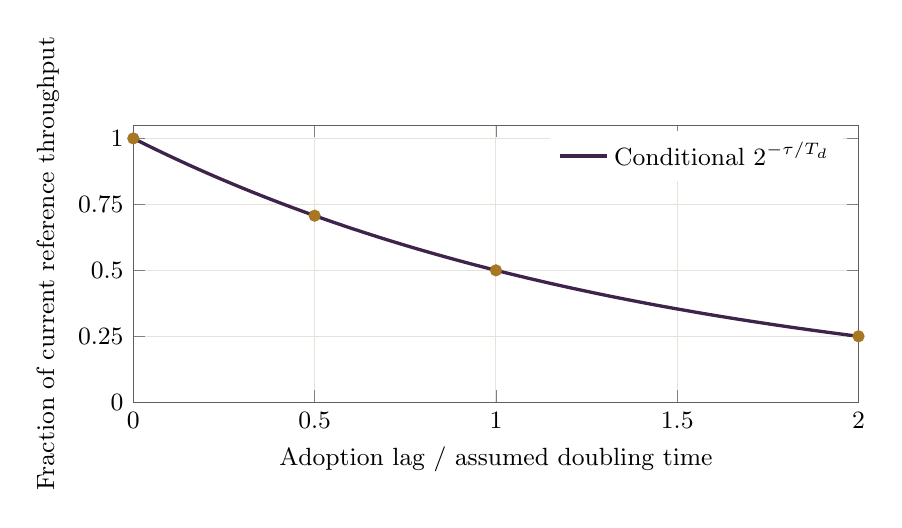
\begin{tikzpicture}
\begin{axis}[width=.89\linewidth,height=5.1cm,xlabel={Adoption lag / assumed doubling time},ylabel={Fraction of current reference throughput},xmin=0,xmax=2,ymin=0,ymax=1.05,xtick={0,.5,1,1.5,2},ytick={0,.25,.5,.75,1},grid=major,grid style={draw=Rule!60},axis line style={draw=Muted},tick label style={font=\small},label style={font=\small},legend style={draw=none,font=\small,at={(.98,.98)},anchor=north east}]
\addplot[very thick,Violet,domain=0:2,samples=80]{2^(-x)};
\addlegendentry{Conditional $2^{-\tau/T_d}$}
\addplot[only marks,mark=*,Gold] coordinates {(0,1)(.5,.70710678)(1,.5)(2,.25)};
\end{axis}
\end{tikzpicture}
\caption{A model of adoption lag, not a forecast. At one assumed doubling time of delay, the institution uses half the current reference throughput; at two, one quarter. Faster adoption only matters when the adopted capability and downstream constraints permit useful conversion.}
\label{fig:lag}
\end{figure}

For a fixed output type requiring construction, validation, delivery, and demand, a stylized pipeline bound is
\begin{equation}
Q(t)\leq\min\{\chi(t)A(t-\tau(t)),\;V(t),\;P(t),\;D(t)\},
\label{eq:pipeline}
\end{equation}
where all terms are measured in compatible accepted-output units. Here $\chi$ is a qualified conversion fraction, $V$ validation capacity, $P$ delivery capacity, and $D$ demand. The minimum is an upper bound under the stated serial requirements, not a universal production function. Better reasoning does not remove a laboratory queue, supplier limit, distribution failure, or unvalidated measurement by itself.

The strategic objective is therefore \emph{shorter evidence-preserving conversion time}, not automatic upgrades. A less capable, cheaper model with a mature instrument can remain the best choice. Rapidly adopting a model that breaks the outcome bridge reduces productive capability even when a public benchmark improves.


\subsection{The conversion contract: a release must change a construction}
A frontier event becomes actionable only when it connects to an executable opportunity. The \emph{conversion contract} binds five records: the exact accessible advance; the previously unresolved construction; the hypothesized change to its limiting condition; the matched experiment; and the artifact whose newly supported use would benefit a successor. The provider's report is evidence about the advance, not evidence for the final link.

This contract makes an important distinction operational. A newly published method can be useful even if its authoring model is unavailable. A publicly documented model can be unusable for a particular account. A model can be accessible yet offer no gain on the relevant construction. Accordingly, discovery and implementation can investigate every promising lead, while qualification applies to the specific executable combination actually tested.

A deployment snapshot should bind model and tool identities, dependency versions, data rights, evaluation version, resource basis, and known provider drift. Where a provider cannot supply a stable model snapshot, that limitation remains in the evidence; a local hash must not masquerade as control over a remote service. An upgrade is adopted for a named capability and scope, rather than silently replacing every qualified component.

The resulting advantage is a hypothesis about \emph{conversion}, not privileged access: two organizations may obtain the same model, but differ in how effectively they identify, construct, validate, distribute, and renew a valuable capability. The experiment must still allow the direct frontier-agent competitor to construct its own means.

\section{Four coupled processes, separately measurable}
\label{sec:loops}
GENESIS connects four processes: external frontier adoption, inventive inheritance, commercial reproduction, and physical expansion. Their coupling is the opportunity; their separation is what makes the account testable.

\textbf{Frontier adoption} imports a useful capability produced elsewhere. \textbf{Inventive inheritance} retains and adapts means constructed by the institution. \textbf{Commercial reproduction} turns accepted delivery into available resources for further work. \textbf{Physical expansion} increases the stock of qualified instruments, production processes, and infrastructure. A successful software campaign may support only one of these.

\subsection{Capability stock, discovery policy, and resources}
Represent an institutional state as
\begin{equation}
S_t=(M_t,\eta_t,H_t,E_t,X_t,L_t,\I_t),
\end{equation}
where $M_t$ is accessible model/tool configuration, $\eta_t$ the discovery policy, $H_t$ the retained capability graph, $E_t$ evidence and exposure history, $X_t$ productive assets and dependencies, and $L_t$ liquid resources after recorded restrictions. Changes in these objects must not be collapsed into a single intelligence score.

A capability record includes executable artifacts, input/output contracts, prerequisites, rights, measured scope, cost, failure modes, and invalidation triggers. An enabling hyperedge links a set of parent capabilities to a successor hypothesis, together with evidence for their contribution. Unsupported compositions remain proposals. Retired methods remain part of history without remaining eligible for deployment.

A valuable intermediate construction need not earn revenue independently. Its justification can be downstream enabling value. But search, failures, verification, transfer, and maintenance still belong in the full account. The institution must also be able to simplify: a smaller archive or a conventional method can outperform a more elaborate self-improving system.

\subsection{A complete-cost condition for useful inheritance}
For $n$ future uses of a specified capability, let $K$ be the one-time acquisition and qualification burden, $c_0$ the complete cost per use without it, and $c_1$ the complete cost per use with it. With equal accepted outcomes and no other changing costs, inheritance pays for itself only when
\begin{equation}
n(c_0-c_1)>K.
\label{eq:reuse}
\end{equation}
This is a transparent accounting condition, not proof that the assumed uses will occur. When costs vary, compare the full discounted or undiscounted sequences under a declared objective. When quality changes, report the change rather than treating every output as interchangeable. A capability can be useful in an individual successor and still fail to recover its programme-wide construction costs.

\subsection{Economic invention is part of the search}
The complete productive arrangement includes the outcome, technical means, acceptance, participants, information, payment, funding, and risk allocation. A cheaper component may create no market if buyers cannot verify it. A different contract may finance a valuable instrument, while introducing obligations that constrain future cash. The technical and economic constructions must therefore inform each other \citep{notes30,superalpha,omegapaper}.

Commercial success does not require a new theorem or an improving model. Repeated, accepted, complete-cost-profitable delivery with collections and feasible reinvestment can constitute a commercial flywheel on its own. The stronger integrated result additionally establishes that retained inventions improve fresh capability construction and help produce subsequent economic value. Neither process should be withheld or declared successful merely because the other succeeds.

\section{The immediate product: a self-service discovery institution}
\label{sec:product}
The initial product is \textbf{GENESIS Discovery Studio}: an installable, local-first application that completes a computational discovery campaign and exports the result, its reproducible evidence, and any supported reusable means. Physical instrument operation is a separately qualified extension. The commercial proposition is customer-owned mission intelligence, not dependence on recurring founder consulting.

\subsection{One user journey, executable underneath}
The opening question is \emph{What should become possible?} The user supplies the objective, authorized sources, resources, and material limits. The application helps expose ambiguities without turning every ordinary computation into an approval request. Once a mission is authorized, routine work within that scope proceeds; material external effects remain controlled.

The interface presents five concrete objects: the mission, competing constructions, actual experiments, supported capabilities, and the successor test. It should show executable artifacts and measured results before conversational traces. A user must be able to distinguish a simulation, a replay of recorded evidence, a new physical measurement, and an accepted commercial delivery without reading a technical appendix.

\begin{table}[htbp]
\caption{First-release contracts. These are proposed product requirements, not implemented endpoints in this publication.}
\label{tab:product}
\begin{tabularx}{\linewidth}{P{2.8cm}YY}
\toprule
\textbf{User action}&\textbf{Executable result}&\textbf{Acceptance evidence}\\\midrule
Launch a campaign&Mission contract, alternatives, resources, and an executable first experiment&Original outcome and complete comparator are explicit; no hidden prerequisite is treated as a fact.\\
Construct the means&Runnable code, representation, procedure, or engineering package&Build and execution logs; dependency and effect checks; development failures retained.\\
Test the candidate&Frozen artifact and protected comparison&Independent outcome checks, uncertainty, all attempts, full resource account.\\
Keep the capability&Portable package with applicability and invalidation rules&New composition and reuse do not inherit unconditional approval.\\
Launch a successor&Fresh construction with and without the claimed inheritance&Matched resources and current models; contribution separated from external model progress.\\
Replay a frontier event&Relevant challenger or justified non-adoption&Verified access and changed obstacle; new confirmation rather than reused holdout.\\\bottomrule
\end{tabularx}
\end{table}

A release should include guided installation, a bundled public example, a resource meter, pause/resume, recoverable execution, clear stop controls, and exportable artifacts. No terminal work or hand-assembled development environment should be required for ordinary use. These are usability tests to pass on supported operating systems, not a promise of universal compatibility before integration.

\subsection{Use public foundations without confusing them with the invention}
Codex's public CLI, SDK, and app-server provide existing agent execution and integration surfaces. The app-server supports persistent threads, streamed events, tools, and approval handling; model access remains separate \citep{codex}. GENESIS should add mission construction, evidence-aware adoption, and successor experiments rather than recreate the runtime. Integrations must be evaluated in the actual environment, not inferred from documentation.

For a non-medical measurement track, FreeCAD provides an open parametric design foundation; EIDORS provides forward and inverse electrical models, including contact-impedance parameters in complete electrode models; and public Finnish EIT data provide recorded measurements and target photographs \citep{freecad,eidors,eidorscem,kitdata}. These are development resources. Recorded observations cannot establish the physical performance of a newly invented acquisition that never occurred.

Commercial EIT16 equipment supports configurable current-injection patterns, multifrequency operation, simultaneous voltage acquisition, and open reconstruction workflows \citep{sciospec}. Those are existing features, not GENESIS inventions. Exact configuration, access, delivery, safety limits, and adapter compatibility require confirmation. Simultaneously acquired voltage channels cannot be counted as saved acquisitions merely because software ignores some of them.

The development policy is to use already available, authorized model and compute access, with no new paid commitments inferred from this paper. A customer-operated release can use its owner's qualified local models or provider account. The seller must not promise unlimited inference under a one-time product price, nor mistake included subscription usage for zero economic resource consumption.

\subsection{Autonomy is an operating result, not a role label}
A campaign is autonomous only over its declared action scope and execution interval. Measure actual human intervention, not hypothetical staff hours copied from a traditional enterprise. Necessary physical assembly, expert adjudication, or external authorization makes the corresponding stage hybrid; normal customer choice remains customer participation rather than hidden internal labor.

Generated code executes in isolated development environments. Credentials and consequential effects pass through externally enforced authority boundaries. The constructor cannot edit its confirmation data, rewrite its resource history, or activate a more permissive controller in order to approve itself. A revised evaluator or controller can be proposed, independently validated, and authorized as a new version. This preserves architectural freedom without circular certification.

The institutional records should distinguish \textbf{world observations}, \textbf{policies}, \textbf{evidence}, and \textbf{authority}. Evidence that a device works does not authorize its operation. Permission to run a test does not make the result true. An engineering hash does not establish either proposition.

\section{How to establish that GENESIS adds value}
\label{sec:evaluation}
The baseline is not an unassisted first answer. Use a tuned specialist, a conventional constructor or optimizer, an unrestricted frontier-agent workflow with the same tools, and an applicable agent-design method. Separate a competent all-human productivity comparator from human-plus-AI competitors and customer self-service. The former measures the human-to-AI productivity opportunity; the latter determine the competitive price and adoption case.

\subsection{Cross external intelligence, inheritance, and discovery}
Let $J(m,h,\eta)$ be an expected terminal campaign outcome under model configuration $m$, initial capability set $h$, and discovery policy $\eta$, with matched complete resources and independent terminal evaluation. A two-level factorial design has eight conditions. Its conditional discovery effect is
\begin{equation}
\Delta_{\eta}(m,h)=\E[J(m,h,\eta_1)-J(m,h,\eta_0)].
\label{eq:factorial}
\end{equation}
Analogous effects isolate $m$ and $h$. Report interactions: a new representation may need a compatible model or constructor. Do not force a joint effect into an additive attribution.

\begin{figure}[htbp]
\centering
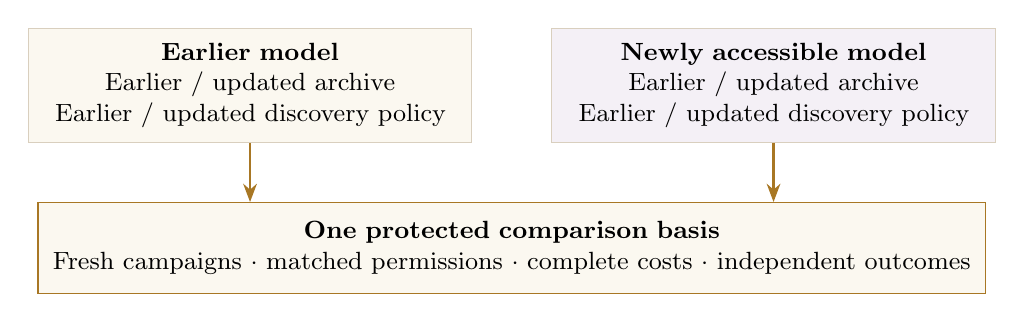
\begin{tikzpicture}[every node/.style={font=\small,align=center},node distance=.4cm]
\node[draw=Rule,fill=Ivory,text width=5.4cm,minimum height=1.45cm] (old) {\textbf{Earlier model}\par Earlier / updated archive\par Earlier / updated discovery policy};
\node[draw=Rule,fill=Pale,text width=5.4cm,minimum height=1.45cm,right=1.0cm of old] (new) {\textbf{Newly accessible model}\par Earlier / updated archive\par Earlier / updated discovery policy};
\node[draw=Gold,fill=Ivory,text width=11.8cm,minimum height=1.15cm,below=.75cm of $(old.south)!.5!(new.south)$] (eval) {\textbf{One protected comparison basis}\par Fresh campaigns $\cdot$ matched permissions $\cdot$ complete costs $\cdot$ independent outcomes};
\draw[-{Stealth},Gold,thick] (old.south)--(old.south|-eval.north);
\draw[-{Stealth},Gold,thick] (new.south)--(new.south|-eval.north);
\end{tikzpicture}
\caption{Eight conditions separate an external upgrade from useful inheritance and a better discovery procedure. Many descendants from one campaign are not independent demonstrations of improved discovery.}
\label{fig:factorial}
\end{figure}

An inherited tool may improve execution without improving invention. To test a generative claim, require construction of a different useful capability rather than another run of the same tool. To test a meta-discovery claim, compare the descendants produced by earlier and revised discovery procedures on independent campaigns. A supplied winning strategy is a diagnostic control, not evidence that the candidate discovered it.

\subsection{Protect confirmation without freezing inadequate measurements forever}
Freeze the candidate, comparator, score, sampling unit, permitted within-episode adaptation, and cost basis before confirmation. Fresh cases must be outside the active builder's development feedback. A disclosed holdout becomes consumed evidence. Cluster related tasks by their actual dependence; hundreds of questions about one source do not yield hundreds of independent campaign replications.

For bounded paired score differences $Y_{t,i}\in[-1,1]$, the foundational manuscript gives a conservative fixed-sample gate \citep{transform}:
\begin{equation}
L_t=\overline{Y}_t-\sqrt{\frac{2\log(1/\alpha_t)}{n_t}},\qquad
\sum_{t\geq1}\alpha_t\leq\alpha.
\label{eq:gate}
\end{equation}
Under the stated conditional independence and freshness assumptions, false promotion across attempts is controlled by the allocated error budget. With separately justified calibration errors $\varepsilon_c,\varepsilon_b$ for candidate and baseline, a practical gain claim needs
\begin{equation}
L_t>\delta+\varepsilon_c+\varepsilon_b.
\end{equation}
This is not a new inequality. The width-two factor is essential. Repeatedly peeking at the fixed-sample bound requires a valid sequential alternative, not a convenient stopping rule. A large sample cannot repair a systematically wrong evaluator. With several prespecified comparisons per attempt, allocate error across both attempt and claim indices; choosing a favorable contrast does not create a fresh error budget. The eight-condition design does not supply eight independent discoveries merely because it has eight cells.

The constructor may invent a better test, but that test is a development artifact until independently validated against the original outcome. An accepted evaluator revision creates a new measurement epoch and compares contenders on a common valid basis. It does not retroactively upgrade earlier results.

\subsection{Negative outcomes are necessary discriminators}
Include cases in which existing methods suffice, the extra observation is uninformative, the proposed explanation set is incomplete, an apparently removable constraint is mandatory, or construction costs cannot be recovered. Reward justified retention and abstention alongside useful change. Penalize both unsupported certainty and indiscriminate refusal. ``No affordable test was found'' is a search-bounded result, not proof that none exists.

Scaling introduces selection pressure: more searches create more opportunities to select a misleading winner. Failed attempts, parallel branches, provider drift, human interventions, and resource exhaustion remain in the campaign history. The sampling unit for improved discovery is the complete campaign, not the agent, token, or candidate.

\section{Executed analytical studies: the links made explicit}
\label{sec:study}
The companion executes five transparent study groups, including release-adversarial cases. They are authored finite or algebraic models, not measurements from a frontier-model campaign. Their purpose is to expose necessary distinctions and provide inspectable construction artifacts. All physical response laws, capability requirements, prices, and costs below are supplied assumptions. The programme makes no network calls and controls no equipment.

\subsection{Construct an observation that removes a genuine ambiguity}
Let the latent state be $\theta=(s,c)$, representing two abstract effects. The installed measurement is
\begin{equation}
y_+=s+c+e_+,\qquad |e_+|\leq\epsilon.
\label{eq:yplus}
\end{equation}
Even with zero noise, $(s,c)=(-2,2)$ and $(2,-2)$ produce the same observation. On the domain $[-2,2]^2$, any estimator using only this observation has worst-case infinity-norm error at least $2$. More reasoning about that observation cannot resolve the ambiguity. Repetition can reduce random noise under appropriate assumptions; it cannot remove this null space.

The supplied construction grammar permits one additional linear observation $y_r=a s+b c+e_r$, where $(a,b)\in\{-1,0,1\}^2\setminus\{(0,0)\}$ and $|e_r|\leq\epsilon$. The constructor enumerates the eight candidates, discards singular observation matrices, and minimizes the exact worst-case noise amplification $\epsilon\|A^{-1}\|_\infty$. Six candidates have full rank. The two signed difference rows attain the best bound. A deterministic tie rule selects $(a,b)=(1,-1)$, yielding
\begin{equation}
\widehat{s}=\frac{y_++y_-}{2},\qquad
\widehat{c}=\frac{y_+-y_-}{2}.
\label{eq:observer}
\end{equation}

\begin{proposition}[An exact, model-relative observation construction]
For the supplied two-effect model with componentwise bounds $|e_+|,|e_-|\leq\epsilon$, the estimator in Equation~\eqref{eq:observer} satisfies $\|\widehat\theta-\theta\|_\infty\leq\epsilon$. Among the eight supplied additional rows, the difference rows minimize that bound. A conventional sum-and-difference constructor achieves the same result.
\end{proposition}
\begin{proof}
The two estimation errors are $(e_++e_-)/2$ and $(e_+-e_-)/2$, so both are bounded by $\epsilon$. The two additional rows parallel to $(1,1)$ are singular. The four coordinate rows have inverse infinity norm $2$; the two difference rows have norm $1$. Thus the claim follows by enumeration of the supplied grammar.
\end{proof}

With $\epsilon=1/10$, exhaustive execution over 25 integer states and nine noise-corner/zero combinations gives 225 cases and worst error $1/10$. The checker independently compares the emitted observer with the conventional algebraic formula. The generated files are \texttt{measurement\_plan.json} and \texttt{compiled\_observer.py}. They implement the abstract response model, not a Sciospec protocol, EIDORS simulation, or fabricated sensor.

A further exact reuse check supplies four new coefficient variants, $y_+=s+kc+e_+$ and $y_-=s-kc+e_-$ for $k=2,3,4,5$. The algebraic constructor produces their estimators and passes 1,764 state/noise checks. Conventional algebra matches. This shows that the supplied constructor works over these variants; it does not demonstrate autonomous cross-domain discovery, reduced search cost, or empirical inventive inheritance.

\begin{statusbox}
\textbf{The decisive failure case.} Add an unmodeled effect $d$ to both observations. Then $\widehat{s}=s+d+(e_++e_-)/2$. At $d=1/2$ and zero noise, error is $1/2$, exceeding the claimed $1/10$ scope. Two equations cannot identify three unrestricted effects. A third explanation cannot be dismissed because the original two-variable model fits its own data.
\end{statusbox}

This witness connects directly to the instrument-invention hypothesis: an obstruction can specify a missing information channel. However, a physical realization must establish that the assumed second response can actually be constructed and calibrated. A proof about a supplied matrix does not provide that bridge. The paper's conventional tie also prevents misrepresenting linear algebra as a new algorithm.

\subsection{Selective replay saves candidate evaluations only under its assumptions}
The finite replay study supplies eight opportunities and four events: a representation capability, a geometry capability, an irrelevant presentation capability, and a measurement capability. Each opportunity has a complete, supplied set of requirements. Success is defined to occur when all requirements are present. A blanket policy retries every unfinished opportunity after every event; a dependency policy evaluates only newly feasible opportunities.

\begin{table}[htbp]
\caption{Exact replay counts in the supplied dependency model. The strong ordinary dependency scheduler ties the selective policy.}
\begin{tabularx}{\linewidth}{Yrrr}
\toprule
\textbf{Policy}&\textbf{Evaluations}&\textbf{Completed}&\textbf{Unresolved}\\\midrule
Retry all unfinished opportunities&25&5&3\\
Selective dependency replay&5&5&3\\
Conventional dependency scheduler&5&5&3\\\bottomrule
\end{tabularx}
\end{table}

The difference is 20 avoided candidate evaluations, not an observed reduction in total discovery cost. Constructing and maintaining the requirement model, routing events, checking access, and discovering omitted dependencies were not modeled. The conventional control is implemented separately: it computes each opportunity's first feasible release from cumulative prefixes, without invoking the selective scheduler. A separate check covers all seven nonempty requirement sets on three capabilities over six release orders: 42 opportunity/order cases agree with independent subset logic. The release tests additionally compare the two implementations over all 256 four-event sequences on a two-capability alphabet, including empty and repeated events.

If an advance changes an unrecorded mechanism, a complete-looking dependency map may miss it. The study therefore supports the arithmetic and the need for relevance routing, not the claim that GENESIS has discovered an optimal replay policy. Real evaluation must price the routing machinery and measure missed opportunities against an equally capable conventional policy.

\subsection{Profit, liquidity, and a funded successor are different quantities}
In a stipulated production episode, setup costs 40 abstract units, each of ten accepted deliveries costs 4, and each pays 12. All declared costs are expensed when paid, all orders are supplied assumptions, and no taxes or other unlisted burdens are claimed to be included. The episode's conditional surplus is
\begin{equation}
\Pi=10\times12-(40+10\times4)=40.
\end{equation}
If each delivery is paid immediately after acceptance, minimum opening cash is 44. If payment for all deliveries occurs only at the end, it is 80. Protecting an additional constant reserve of 10 raises the first requirement to 54. Identical profit does not imply identical financeability.

\begin{proposition}[Exact funding requirement for an ordered cash plan]
For cash increments $x_1,\ldots,x_T$ and protected reserve $r_t\geq0$ at each prefix $t=0,\ldots,T$, the minimum nonnegative opening cash is
\begin{equation}
B_{\min}=\max\left\{0,\max_{0\leq t\leq T}\left(r_t-\sum_{u=1}^{t}x_u\right)\right\}.
\label{eq:capital}
\end{equation}
\end{proposition}
\begin{proof}
Every prefix requires $B+\sum_{u=1}^{t}x_u\geq r_t$. Rearranging all inequalities gives the necessary lower bound; choosing their maximum satisfies all of them. This proves sufficiency as well.
\end{proof}

The companion compares Equation~\eqref{eq:capital} with independent brute-force funding checks on 1,440 schedules. It also verifies a second stipulated episode: setup 30, five deliveries costing 4 and paying 12, with immediate collection. That episode needs 34 opening units and earns 10. The first episode's fully collected surplus of 40 can therefore fund it while preserving the original seed; the earned-resource pool becomes 50. This is an exact financial continuation under assumptions, not evidence that the first invention caused the second or that any customer exists.

Negative cases matter. With only three orders, the first episode loses 16; non-entry is preferable. At price 8 for ten orders, its surplus is zero, so no additional invention can be funded from its earnings. An unmodeled lifecycle burden greater than 40 erases its apparent surplus. A conventional provider with the same construction and transactions has the same economics.


\subsection{Adversarial replay: when the attractive policy should lose}
\label{sec:adversarial}
A publication intended to guide operation needs counterexamples to its most attractive mechanism. The new companion adds three exact, authored checks. First, announcing a solver does not add it to the accessible capability set. Second, removing access suspends current eligibility while preserving historical qualification. Restoring access can restore logical feasibility, but a real system must separately re-establish operational validity. This finite state machine models neither authentication nor an actual deployment controller.

Third, a supplied blocker index says that a task requires an old solver, while the actual supplied routes also admit a new representation. An event makes that representation available. The rigid index selects nothing although a valid route exists. The example implements the limitation discussed in Appendix~\ref{app:derivations}: a system intended to reopen possibilities can miss them by treating its own dependency map as final.

There is also a precise economic correction. Let $N_b$ and $N_s$ be candidate-evaluation counts for blanket and selective replay, let $c_e$ be a common cost per evaluation, let $K_r$ include the incremental cost of constructing and operating the routing policy, and let $L_m$ be the net accepted value forgone by its missed opportunities relative to the comparator. Under this accounting model,
\begin{equation}
G_{\mathrm{replay}}=(N_b-N_s)c_e-K_r-L_m.
\label{eq:replay-net}
\end{equation}
This is a conditional accounting identity, not an estimator of an unknown opportunity portfolio. A reduction in evaluations is insufficient for an advantage. For the supplied counts $25$ and $5$ and $c_e=1$, the three scenarios are:
\begin{center}
\small
\begin{tabular}{lrrr}
\toprule
\textbf{Authored scenario}&$K_r$&$L_m$&$G_{\mathrm{replay}}$\\\midrule
Low routing burden&3&0&17\\
Expensive routing&25&0&$-5$\\
Missed valuable alternative&3&30&$-13$\\\bottomrule
\end{tabular}
\end{center}
All values are abstract, stipulated units, not measured commercial savings. The result sharpens the invention target: improve the ability to find relevant new constructions \emph{after} routing costs and missed possibilities, not merely reduce the number of retries. An exploration allocation can be justified, but its size is another policy to test, not a universal constant.

\subsection{What the computations establish}
\begin{table}[htbp]
\caption{Executed result ledger. All results are exact within supplied finite models or conditional algebra; none is a new physical or commercial observation.}
\label{tab:results}
\begin{tabularx}{\linewidth}{P{3.2cm}YY}
\toprule
\textbf{Study}&\textbf{Established}&\textbf{Not established}\\\midrule
Observation construction&Eight rows evaluated; six full-rank; 225 noise/state checks; best error bound $0.1$.&An autonomously invented physical information channel or superiority over ordinary algebra.\\
Supplied constructor reuse&Four coefficient variants; 1,764 exact checks.&Cross-domain discovery, measured construction savings, or a stronger inventor.\\
Frontier replay&25 versus 5 candidate evaluations; same five completions; independently executed ordinary tie.&Complete-cost advantage, accurate real-world relevance detection, or a new scheduler.\\
Financial continuation&44 versus 80 opening units; surplus 40; conditional successor funded from earnings.&Demand, actual collections, native enterprise operation, or actual profit.\\
Adoption lag&The stated exponential assumption gives $2^{-\tau/T_d}$.&A measured law of AI progress, an adoption forecast, or exponential enterprise growth.\\\bottomrule
\end{tabularx}
\end{table}

Sixty-eight analytical and release-integrity tests pass in the delivered environment, under both normal and optimized Python execution. This checks specified code and arithmetic, not the proposed foundry's empirical efficacy. The strength of the package is that a reader can reproduce the distinctions, inspect the ordinary ties, and identify exactly what the next scientific experiment must add.

\section{The commercial design: make capability easy to buy and use}
\label{sec:commerce}
The first commercial hypothesis is a self-service, customer-owned discovery application with portable campaign artifacts and qualified domain packages. Buyers operate their own authorized compute and evidence. The seller's advantage should be better complete outcomes, easier successful use, reliable construction, and supported capability inheritance---not dependence on the founder to interpret every run.

The product should not require a promise of unlimited updates or personal support. An acquired edition remains usable within its supported environment. Optional later editions and newly qualified capability packages must earn their price through measured value. Embedded documentation and local assistance should handle ordinary use; the costs of failures, refunds, security maintenance, and any support actually provided remain visible. Removing personal consulting does not make those obligations disappear.

\subsection{The price window is an invention specification}
Under a quasilinear participation model in common monetary-equivalent units, let $v_i$ be buyer $i$'s expected value of the accepted outcome, $u_i^{\rm out}$ the utility of its best available alternative, and $b_i$ the buyer's non-price burden: compute, setup, attention, integration, risk, and remaining verification. Participation requires
\begin{equation}
p_i\leq v_i-u_i^{\rm out}-b_i.
\label{eq:buyer}
\end{equation}
For $n$ deliveries with fixed lifecycle burden $F$, per-delivery cost $c$, and required total surplus $m$, a common price needs
\begin{equation}
p\geq c+\frac{F+m}{n}.
\label{eq:seller}
\end{equation}
Together these conditions identify what must change: lower a complete cost, improve accepted value, reduce buyer burden, or reach additional genuine demand. Increasing $n$ is not legitimate unless buyers, capacity, acquisition, and obligations support it. Reducing the buyer's outside-option cost can shrink the allowable price even while our production improves.

These inequalities are feasibility conditions, not incentive-compatibility or equilibrium proofs. A claim of game-theoretic optimality must specify participants, feasible actions, information, strategic responses, timing, and an exact solution or justified bound. Buyers may decline. Suppliers may raise prices. Competitors may adopt the same model or construct the same tool. The system must be able to choose non-entry.

\subsection{Invent the complete arrangement}
A capability may be sold as software, a qualified workflow package, a licensed process, or a shared instrument arrangement. Those are hypotheses to compare, not a compulsory catalogue. Construction and transaction design interact: a method that makes performance measurable can enable a different acceptance contract; staged delivery can reduce working-capital needs; a standard interface can make distribution economical. Customer prepayments can provide cash but remain obligations until earned.

The closed commercial episode is
\begin{center}
\small\textbf{Offer $\rightarrow$ voluntary choice $\rightarrow$ funded order $\rightarrow$ actual production $\rightarrow$ independent acceptance $\rightarrow$ collection $\rightarrow$ obligations covered $\rightarrow$ available reinvestment.}
\end{center}
An invoice is not collection. Financing is not revenue. Accounting profit is not unrestricted cash. A successful simulation is not a customer. These distinctions follow the author's economic research and must persist through autonomous execution \citep{notes30,notes29,omegapaper}.

Report the complete cost vector before converting it into money: model and tool use, elapsed time, compute, data acquisition, construction, failed searches, checking, packaging, distribution, actual human work, support, maintenance, financing, and remaining obligations. Subscription access is not evidence of free production. Conversely, do not impose fictional human review on a genuinely autonomous task merely because the human comparator uses it.

\subsection{Scale is a consequence of unit value, distribution, and renewal}
A large addressable industry does not establish obtainable orders. The first commercial test is an accepted paid use with measured buyer benefit and complete seller economics, followed by repeated self-service success. Distribution should expand only where incremental acquisition and delivery remain worthwhile. Prices need not be anchored to a fixed discount or a maximum conversion rate.

The lab's public research programme retains an unachieved objective of US\$3 billion in trailing-365-day complete-cost profit, with starting capital treated as a joint strategy-and-financing choice for new work \citep{labreadme}. This is a milestone, not a forecast, ceiling, or reason to assume funding. A scale identity is useful only as a requirement: at complete-cost margin $\mu>0$, annual revenue must be $3\text{ billion}/\mu$. At an illustrative $\mu=0.5$, that is US\$6 billion. Neither the margin nor the demand is observed here.

The durable commercial question is not whether a model can generate a deliverable cheaply once. It is whether the institution can repeatedly deliver outcomes buyers prefer, withstand changing alternatives, and renew its productive advantage before it becomes uneconomic. Frontier Replay is valuable when it helps that renewal after its own costs; ordinary delivery and distribution can remain the best next investments.

\section{The first physical track: an instrument, not a scanner story}
\label{sec:physicaltrack}
A concrete prospective mission asks whether an observed electrical response changed because of a sample's interior, the electrode contact, both, or another disturbance. The construction target is a usable discriminating observation, not merely a sharper reconstruction image. It could involve geometry, a supported excitation, a reference intervention, calibration, analysis, or a combination. The winner is not supplied exclusively to the candidate.

The installed comparison must include strong inverse methods, contact-aware modeling, uncertainty analysis, existing measurement configurations, and competent alternative construction. Each gets the same meaningful permissions to reposition, recalibrate, select supported frequencies, or procure suitable means. If an ordinary complete route already meets the requirement, the alleged residual must be revised.

Use public recordings for regression and appropriately calibrated simulation for candidate exploration. The original acquisition geometry and noise provenance remain attached to the data. A new physical-information claim requires new measurements on independently prepared cases, including combined effects and cases outside the original explanation set. Suitable simulation does not establish a manufactured fixture's tolerances, electrode behavior, or long-term reliability.

The proposed physical package contains dimensioned CAD, an implementable connection map, a restricted acquisition specification, calibration software, an interpretation program with abstention, and independent evidence. It is tank-only and non-medical at first. Human mounting or fabrication is disclosed as such; the product does not become fully autonomous because those steps occur outside a screenshot.

A prospective successor should test a different consequential measurement problem. It may inherit a calibrated component, fixture-construction method, or experimental-design procedure, but must re-establish compatibility. Holding the model fixed isolates inheritance; allowing a control to build or buy its own means avoids a contrived advantage. This track earns flagship status only through a meaningful new capability or affordability threshold, not by being the first experiment with available code.

\section{From a useful instrument to a larger productive civilization}
\label{sec:horizon}
The long horizon is not a larger chatbot business. It is an institution whose intellectual and commercial achievements can finance and construct expanding scientific and industrial capacity. The relevant chain can begin with a modest instrument yet reach far beyond its initial field: better observations support better process models; those models support productive methods; productive methods support energy and manufacturing; those assets make more capable instruments and infrastructure affordable.

No single chain is mandatory. Intermediate constructions can be jointly enabling, and a later discovery may replace the original route. What matters is that each arrow names a real dependency, an executable construction, an accepted outcome, and the resources that permit continuation.

\begin{table}[htbp]
\caption{A prospective ladder of productive expansion. Rows describe research horizons, not achieved GENESIS capabilities or dated forecasts.}
\label{tab:ladder}
\begin{tabularx}{\linewidth}{P{2.8cm}YY}
\toprule
\textbf{Frontier}&\textbf{Means to construct}&\textbf{Evidence before scaling}\\\midrule
Scientific observation&New instruments, calibration, discriminating experiments&Independent physical uncertainty and useful decisions beyond complete alternatives.\\
Materials and processes&Qualified processing, separation, control, and manufacturing methods&Yield, energy per conforming unit, reliability, lifecycle cost, accepted demand.\\
Productive infrastructure&Systems able to construct and maintain useful tools and components&Net qualified output after maintenance, replacement, logistics, and protected obligations.\\
Energy abundance&Better generation, storage, conversion, distribution, and heat management&Useful delivered energy and full resource accounting; no assumed energy or material surplus.\\
Space-based industry&Robotic construction, resource processing, repair, and infrastructure&Mission-specific tests of transport, production, reliability, governance, and economics.\\
Stellar-scale productive reach&Distributed energy collection and industry supported by preceding capacities&Physical throughput, material supply, heat rejection, coordination, and durable public benefit.\\\bottomrule
\end{tabularx}
\end{table}

\FloatBarrier
\subsection{Physical capacity cannot be replaced by financial notation}
Let $K$ denote a specific stock of qualified productive units. A simplified necessary accounting relation is $\dot K=b-d$, where $b$ is build rate and $d$ retirement or loss rate. If each new unit needs energy $E_K$, material $M_K$, fabrication capacity, and qualification, then
\begin{equation}
b\leq\min\left\{\frac{P_{\rm available}}{E_K},\frac{\dot M_{\rm available}}{M_K},\ b_{\rm fabrication},\ b_{\rm qualification}\right\}.
\label{eq:physical}
\end{equation}
This dimensional bound assumes those inputs are required and available in the specified form. Better discovery may change the coefficients or invent a different process. It cannot simply book missing materials, spare parts, or energy as future profits. Positive net expansion requires $b>d$ and a feasible sequence of intermediate commitments, not merely a favorable terminal spreadsheet.

The IAU nominal solar luminosity is $L_\odot^{\rm N}=3.828\times10^{26}$ W, a conversion constant rather than a claim about instantaneous solar output \citep{iau}. A hypothetical infrastructure intercepting fraction $f$ and using conversion efficiency $\eta_E$ before separately metered parasitic loads would have the dimensional scale
\begin{equation}
P_{\rm useful}=\eta_E f L_\odot^{\rm N}-P_{\rm parasitic}.
\label{eq:stellar}
\end{equation}
At $f=10^{-8}$, the intercepted power scale before conversion is $3.828\times10^{18}$ W. This arithmetic is neither a design nor an attainable near-term target. It identifies how large the ultimate productive horizon is relative to the first instrument, while leaving every physical dependency explicit.

NASA's space-based solar-power analysis already identifies substantial launch, manufacturing, and assembly challenges in far smaller prospective systems \citep{nasa}. GENESIS would have to contribute actual enabling advances, not assume those constraints vanish. Materials, heat rejection, ecological consequences, resilience, institutional legitimacy, and the distribution of benefits remain design requirements.

The route to extraordinary enterprise value is therefore not an assertion that owning intelligence guarantees a claim on all future wealth. It is repeated creation of additional value, voluntary participation, sustainable value capture, and reinvestment into means that expand useful production. Competitive diffusion can benefit civilization while reducing a particular seller's margin. A durable institution must accommodate that possibility rather than depend on permanent scarcity of model access.

\begin{thesisbox}
\textbf{Civilization-scale ambition begins with an evidence-scale step: construct one missing means, establish what it enables, and make the next consequential construction genuinely easier or more affordable.}
\end{thesisbox}

\section{The decisive programme}
\label{sec:programme}
The next empirical result should be a complete construction campaign, not another architecture diagram. Select the opportunity for its enabling consequence, not because its evaluator is convenient. Compare materially different opportunities before commitment; preserve promising physical and economic hypotheses without promoting them prematurely.

The first release target is one autonomous computational campaign that delivers a usable capability and a fresh successor experiment. The first physical result requires new measurements. The first commercial result requires a genuine accepted, collected delivery. The first improved-inventor result requires campaign-level evidence with the underlying model and starting capability stock controlled. These milestones can progress in parallel and fail independently.

\begin{table}[htbp]
\caption{Research decisions that can reject the proposed advantage.}
\begin{tabularx}{\linewidth}{P{2.3cm}YY}
\toprule
\textbf{Claim}&\textbf{Required test}&\textbf{Disconfirming result}\\\midrule
Useful construction&Complete outcome versus strong, equally permitted routes&The ordinary route already meets the same outcome more economically.\\
Frontier conversion&New accessible capability revisits a recorded obstacle and passes fresh confirmation&The upgrade adds no relevant accepted capability or breaks the existing bridge.\\
Inheritance&Fresh successor with and without retained means, including all costs&The gain disappears after transfer, maintenance, or equal construction permissions.\\
Improved discovery&Earlier and revised policies across independent matched campaigns&Only the newer model or richer initial archive explains the gain.\\
Commercial viability&Self-service buyer success, actual acceptance and collections&Acquisition, failures, obligations, or competitive alternatives erase surplus.\\
Physical expansion&Qualified assets produce more useful capacity than they consume or lose&Replacement, energy, material, or qualification constraints prevent net expansion.\\\bottomrule
\end{tabularx}
\end{table}

No fixed agent count, field catalogue, business size, or arbitrary revenue ceiling defines the mission. Each registered experiment nevertheless needs real finite resources, valid stopping conditions, and recovery behavior. A bounded test is not a ceiling on the enterprise; unlimited ambition is not spendable cash, unlimited compute, or authority to act.

The supplied historical Strategy Laboratory reports local strategy search, fresh confirmation, and retention or rejection in route, scheduling, and evidence-selection tasks. It explicitly did not use a live frontier-model proposer in those runs \citep{notes18}. That historical report supports a starting engineering direction, not the integrated GENESIS claim. This edition neither reruns that original package nor relabels its results as new achievements.

The public lab record likewise distinguishes simulated operation from actual revenue and keeps the current Blue Sky flagship unestablished \citep{labreadme}. Our new contribution is the synthesis, the frontier-coupled product and experiment design, and the transparent calculations delivered here. These should guide construction; they must not substitute for it.

\Needspace{28\baselineskip}

\section{Release engineering: publish the research, qualify the operation}
\label{sec:release}
A publication is not an operating institution. Reproducing a calculation does not establish that a customer can install and operate GENESIS Discovery Studio. This release supplies a publication pathway and a separate operational admission contract.

\subsection{What can ship in this edition}
The release contains the paper, editable source, analytical companion, results, tests, claim register, and reading guide. Its static site needs no live model, credentials, backend, analytics tracker, or device connection. The arithmetic explorer illustrates the supplied model; it is not a discovery agent or sensor.

The verifier checks the complete file inventory, hashes, local links, regenerated outputs, and tests. Full verification rebuilds with shell escape disabled, rejects LaTeX warnings, and compares extracted text with the inspected PDF. Tests execute the emitted observer, compare a separately implemented conventional scheduler, and retain essential checks under optimized Python.

Hashes establish consistency, not publisher identity: replacing both files and manifest preserves internal consistency. Origin assurance requires a trusted distribution channel or digest. These checks are not external security or scientific certification. Original numerical results and correction history remain preserved.

\subsection{The operational contract that the product must earn}
A prospective computational pilot should bind
\begin{equation}
\mathcal D=(a,\I,E,M,T,P,R,\ell),
\end{equation}
where $a$ identifies the exact executable release; $\I$ its mission; $E$ the qualified evaluator; $M,T$ the available models and tools; $P$ the enforced permissions; $R$ the resource and recovery policy; and $\ell$ the supported deployment scope and renewal conditions. This is a specification, not an implemented permit system in the companion.

\begin{table}[htbp]
\small
\caption{Release states must not borrow evidence from one another. Product and physical rows are admission requirements, not achievements of this package.}
\begin{tabularx}{\linewidth}{P{2.4cm}YY}
\toprule
\textbf{Release scope}&\textbf{Evidence needed}&\textbf{Permitted public claim}\\\midrule
Research publication&Readable rendered paper, working links, source provenance, clean rebuild, exact study reproduction.&A research manuscript with reproducible analytical examples.\\
Computational pilot&Actual installed campaign, available model, isolated execution, measured resources, interruption recovery, independent result checks.&A bounded discovery workflow operated on the named tasks.\\
Reusable capability&Fresh comparison, valid scope, complete costs, current dependency checks.&The named capability achieved the reported outcome in scope.\\
Improved inventor&Fresh campaign-level comparison with model and initial archive controlled; actual descendant construction.&The changed construction procedure improved the measured campaign outcome.\\
Physical / commercial use&Appropriate new physical evidence or actual accepted and collected delivery, plus separately applicable operating requirements.&Only the physical or economic result actually observed.\\\bottomrule
\end{tabularx}
\end{table}

Before a pilot, test holdout isolation, evaluator substitution, unauthorized effects, resource accounting, duplicate settlement, interruption recovery, and rollback. Enforce builder/verifier separation through processes and storage, not prompts alone. Exercise actual providers, supported operating systems, and the browser-to-executor path. Routine authorized work should proceed without repeated approvals; new permissions cannot arise from a model's proposal.

\subsection{The first paid promise must match the shipped artifact}
The research package must not be sold as a functioning autonomous foundry. The prospective software offer is a usable campaign with declared inputs, accepted outputs, supported environments, failure handling, and exportable evidence. Customer experiments must test that outcome and its adoption burden, not enthusiasm alone.

Distinguish \emph{available now}, \emph{tested scope}, and \emph{research target}. Disclose inference access, equipment, commercial terms, and continuing obligations. Promise neither universal superiority nor guaranteed profit. The ambition remains substantial: make consequential investigation easier to commission, execute, trust, retain, and improve than the strongest feasible alternative.

\section{Conclusion: build the advantage that builds the next advantage}
\label{sec:conclusion}
The frontier of AI is increasingly a source of constructible means. The strategic opportunity is to turn that source into an institution that can preserve mission, replace models, test new capabilities, and learn which constructions deserve to survive. The institution must do more than accumulate knowledge or generate hypotheses: it must change what can be investigated, produced, and economically sustained.

ALPHA GENESIS FLYWHEEL $\Omega$ gives this ambition an operating form. Alpha selects consequential possibilities. The Gym develops competing constructions. Protected qualification binds claims to evidence. SUCCESSOR $\Omega$ preserves useful means while renewing their validity and authority. Frontier Replay connects new external capabilities to the unresolved obstacles they might remove. Commercial operation funds continuation without requiring every profitable action to improve intelligence.

The strongest result would not be one spectacular invention. It would be a supported lineage: a useful construction, an improved fresh successor, a better method of constructing further successors, and a sustainable economic path that expands real productive capacity. The proposed programme keeps that horizon open without treating it as already achieved.

\begin{thesisbox}
\begin{center}
{\Large\bfseries\color{Violet}ALPHA GENESIS FLYWHEEL $\Omega$}\par\medskip
\textbf{Turn the next advance in AI into your next ability\\to autonomously discover at scale.}\par\medskip
New intelligence. New means. Verified outcomes. Stronger successors.\par\medskip
\textbf{Build the advantage that builds the next advantage.}
\end{center}
\end{thesisbox}

\clearpage
\appendix
\section{Reproduction and delivered artifacts}
\label{app:reproduce}
The companion uses Python's standard library and exact rational arithmetic for the finite observation and cash studies. The lag example uses ordinary floating-point evaluation of its stated algebra. It makes no provider calls, performs no network downloads, operates no hardware, and creates no business accounts. No credentials are required.

From the extracted source-package directory:
\begin{lstlisting}
python3 -m unittest discover -s study -p 'test_*.py' -v
python3 study/companion.py --output /absolute/new/genesis-results
\end{lstlisting}
For the checked release path, run \texttt{python3 verify.py}; add \texttt{--full} to rebuild and compare the paper. The output directory must not already exist. This preserves earlier evidence rather than silently overwriting it. Compare the new \texttt{results.json} with \texttt{study/results/results.json}. The programme also emits the abstract measurement plan, executable observer, and lag CSV. The JSON contains explicit scope statements.

To build the paper with a normal TeX Live installation:
\begin{lstlisting}
pdflatex -no-shell-escape -interaction=nonstopmode -halt-on-error \
  ALPHA_GENESIS_FLYWHEEL_OMEGA.tex
pdflatex -no-shell-escape -interaction=nonstopmode -halt-on-error \
  ALPHA_GENESIS_FLYWHEEL_OMEGA.tex
\end{lstlisting}
The bibliography is embedded, so BibTeX is not required. The paper uses New PX fonts, TikZ/PGFPlots, tcolorbox, and standard LaTeX packages. The complete source package includes its author-supplied visual reference. A standalone source build without that image uses a clearly labeled fallback. The release verifier rejects a missing bundled image. No font files are distributed.

\begin{table}[htbp]
\caption{Package map. The study is an analytical companion, not a functioning discovery product.}
\begin{tabularx}{\linewidth}{P{5.0cm}Y}
\toprule
\textbf{File or directory}&\textbf{Purpose}\\\midrule
Root PDF&Inspected compiled paper.\\
Root LaTeX source&Editable manuscript, vector figures, equations, and bibliography.\\
\path{study/companion.py}&Reproducible observation, replay, cash, and lag studies.\\
\path{study/test_*.py}&Analytical, adversarial, emitted-artifact, and publication-integrity checks.\\
\path{study/results/}&Retained exact results and generated abstract observer.\\
\path{source/} provenance&Input identities and non-redistribution status of private research files.\\
\path{source/} source register&Primary-source addresses, inspection date, and evidential use.\\
\path{README.md}, reading guide&Build, reproduction, scope, and reading instructions.\\
\path{SHA256SUMS}&Checksums of delivered package contents, excluding the checksum file itself.\\\bottomrule
\end{tabularx}
\end{table}

\section{Source lineage and claim boundaries}
\label{app:source}
The three author-supplied DOCX files are research conversations containing proposals, corrections, and historical reports. They are not interchangeable with independently reproduced experiments. The \emph{Transformational Intelligence} PDF and its LaTeX source supply the formal foundation. The supplied posters contribute the four-stage vocabulary, ownership framing, and visual identity. This edition introduces the GENESIS synthesis and labels its own computations separately.

\begin{table}[htbp]
\small
\caption{How the supplied sources enter this edition. Page numbers refer to the supplied rendered documents.}
\begin{tabularx}{\linewidth}{P{3.4cm}YY}
\toprule
\textbf{Source}&\textbf{Material carried forward}&\textbf{Boundary retained}\\\midrule
\emph{Transformational Intelligence}, 24 pp.&Purpose/formulation/evaluation (pp.~3, 6--7); architecture (p.~10); confirmation and calibration (pp.~20--22).&Its exact causal example is a supplied-model result, not a measured general inventor.\\
30 October collection \citep{notes30}&Structural transfer, invention of missing means, capability networks, separate commercial and inventive loops; productive-arrangement synthesis.&Conversations propose mechanisms and discuss conditional results; they do not establish open-ended autonomous discovery or actual profit.\\
29 October collection \citep{notes29}&Executable transformations, mutable discovery policy, generative inheritance, complete-cost comparison, and autonomy-cost corrections.&A richer initial tool is not evidence of a better discovery process; human work is charged when actually required.\\
18 October collection \citep{notes18}&Source-grounded adversarial checking and the reported Strategy Laboratory (pp.~7--11).&Reported local algorithmic experiments; no live frontier-model calls in those runs, and no re-execution here.\\
Supplied SUCCESSOR $\Omega$ visuals&Alpha, Gym, Specialist ASI, and institutional continuity; gold/ivory/violet design language.&Concept art and project terminology, not certification, scientific data, or measured superiority.\\\bottomrule
\end{tabularx}
\end{table}

The supplied manuscripts distinguish commercial reproduction from invention. The present paper preserves that distinction and adds an external-frontier axis. It does not impose a permanently fixed agent hierarchy, demand that every useful component be novel, or treat the sensing example as an immutable business choice. It also preserves the right of an ordinary method to win.

\textbf{Public-source snapshot.} The lab README was inspected on 4 November 2026, with returned Git blob identity \texttt{ada27d867a7584bb581fcb65b784141413a5d4aa}. This is a file identity, not a repository commit or a certification of every linked experiment. The package records source URLs and access dates; mutable pages may change after the cutoff.

\textbf{Novelty and review.} No priority claim is made for linear inverse design, dependency scheduling, capital-prefix accounting, exponential lag arithmetic, or statistical concentration. The contribution is their mission-relative connection to frontier adaptation, generative inheritance, and economically sustained discovery. This edition has not received external peer review. The analytical companion checks the declared constructions, not the validity of every physical or commercial assumption.

\textbf{AI assistance and authorship.} Prepared for Vincent Boucher using an AI-assisted research, drafting, coding, and typesetting workflow. The author-supplied mission and manuscripts are the intellectual basis; newly introduced analyses and proposals are presented as such. External empirical claims are attributed to their sources. No private source dialogue is redistributed in the package.

\section{Additional derivations and counterexamples}
\label{app:derivations}
\subsection{Why identical evidence cannot be repaired by a stronger model}
Suppose two possible states $\theta_0,\theta_1$ induce the same distribution over every authorized observation transcript under the installed observation procedure. Any estimator, including one implemented by a stronger language model or multiple interacting agents, is a function of that transcript and additional randomness. If that randomness and initial information are independent of the hidden state, the estimator's output distribution is also the same under both states. Under equal prior mass and binary forced choice, expected accuracy is therefore $1/2$. Abstention cannot increase unconditional correct-identification probability. This is the same informational distinction illustrated in the foundational manuscript \citep{transform}.

For the deterministic pair in Section~\ref{sec:study}, any common estimate must be at infinity-norm distance at least half the separation between the two states, giving the error lower bound $2$. The added response changes the information, not the power of reasoning about an unchanged transcript. Its physical realizability is a separate premise.

\subsection{A conditional commercial value of reducing adoption lag}
Suppose a qualified capability can serve a constant rate $d$ of actual demanded deliveries, with contribution per accepted delivery $m_0e^{-\lambda t}$ as competition erodes the margin. Let adoption lag be $\tau$, horizon $T>\tau$, and one-time adoption cost $K$. Under this deliberately simple model, undiscounted contribution after adoption is
\begin{equation}
W(\tau)=\begin{cases}
\dfrac{d m_0}{\lambda}\left(e^{-\lambda\tau}-e^{-\lambda T}\right)-K,&\lambda>0,\\[5pt]
dm_0(T-\tau)-K,&\lambda=0.
\end{cases}
\end{equation}
The derivative for fixed $K$ is $-dm_0e^{-\lambda\tau}$. Earlier qualified adoption has value when the assumptions hold. But if reducing lag changes $K$, reliability, demand, or future obligations, the sign of the complete investment comparison must be recalculated. A shorter unsafe or invalid qualification process is not a legitimate economic improvement. This is target arithmetic, not a measured demand or margin-decay model.

\subsection{A replay index is not a complete theory of possibility}
Under the finite study's complete prerequisite sets $R_j$ and monotonically expanding available set $A_t$, the predicate $R_j\subseteq A_t$ exactly determines its stipulated feasibility. A dependency scheduler can therefore avoid evaluation while that predicate is false. This is an ordinary logical implication. In a real campaign, $R_j$ can be incomplete, a model may bypass a supposed prerequisite, or access may deteriorate. Then the implication is not justified. The policy must permit diagnostic exploration, revision of the prerequisite model, and revalidation after non-monotone changes.

This counterexample prevents a subtle failure of Frontier Replay: a system designed to reopen blocked possibilities can become a new restriction if it regards its own blocker map as final. Transformational intelligence must be able to challenge the representation used to decide what is worth revisiting.

\clearpage
\begin{thebibliography}{99}
\small\raggedright
\bibitem{transform} Vincent Boucher. \emph{Transformational Intelligence: Learning to Change the Game}. MONTREAL.AI, October 2026. Author-supplied research manuscript, 24 pages, with matching LaTeX source. See Appendix~\ref{app:source}.
\bibitem{notes30} Vincent Boucher. \emph{AGI ALPHA research dialogues: structural discovery, recursive invention, and productive economic arrangements}. Author-supplied research source A, inspected 4 November 2026. Unpublished contextual material; historical claims not independently reproduced here.
\bibitem{notes29} Vincent Boucher. \emph{Transformational architecture and autonomous commercial flywheels}. Author-supplied research source B, inspected 4 November 2026. Unpublished contextual material.
\bibitem{notes18} Vincent Boucher. \emph{Adversarial strategies and SUCCESSOR $\Omega$ Strategy Laboratory}. Author-supplied research source C, inspected 4 November 2026. Unpublished report of earlier local experiments.
\bibitem{engineering} OpenAI. \emph{Accelerating engineering for the physical world}. 3 November 2026. \url{https://openai.com/index/accelerating-engineering-for-the-physical-world/}. Accessed 4 November 2026.
\bibitem{chemistry} Zoi Tsangalidou, Ruijie (Kelly) Zhang, Sukhdeep Singh, and Michael V. LeVine. \emph{Agentic cheminformatics with Google Antigravity}. Google DeepMind, 3 November 2026. \url{https://deepmind.google/blog/agentic-cheminformatics-with-google-antigravity/}. Accessed 4 November 2026.
\bibitem{era} Google Research. \emph{Empirical Research Assistance (ERA): From Nature publication to catalyzing Computational Discovery}. 19 May 2026; MCP availability update 3 November 2026. \url{https://research.google/blog/empirical-research-assistance-era-from-nature-publication-to-catalyzing-computational-discovery/}. Accessed 4 November 2026.
\bibitem{hyperagents} Jenny Zhang, Bingchen Zhao, Wannan Yang, Jakob Foerster, Jeff Clune, Minqi Jiang, Sam Devlin, and Tatiana Shavrina. \emph{Hyperagents}. arXiv:2603.19461v2. Revision registered 1 November 2026; manuscript title page dated 3 November 2026. \url{https://arxiv.org/abs/2603.19461v2}.
\bibitem{modelnotes} OpenAI. \emph{Model Release Notes}. Entries for 26 October 2026 (GPT-6.1 Terra) and 30 October 2026 (GPT-6 Rosalind Research). \url{https://help.openai.com/en/articles/9624314-model-release-notes}. Accessed 4 November 2026.
\bibitem{biology} OpenAI. \emph{Using thousands of AI agents to uncover new leads in biological data}. 21 October 2026. \url{https://openai.com/index/scaling-ai-research-for-complex-biological-data/}. Accessed 4 November 2026.
\bibitem{openaimath} OpenAI. \emph{Mathematical manuscripts and supporting proof artifacts}. Public repository, README and collection snapshot inspected 4 November 2026. \url{https://github.com/openai/math/tree/4eaee87548250b2682affda7d05d947c05554bae}.
\bibitem{alphaevolve} Alexander Novikov et al. \emph{AlphaEvolve: A coding agent for scientific and algorithmic discovery}. arXiv:2506.13131, 2025. \url{https://arxiv.org/abs/2506.13131}.
\bibitem{adas} Shengran Hu, Cong Lu, and Jeff Clune. \emph{Automated Design of Agentic Systems}. arXiv:2408.08435v2, 2025; original submission 2024. \url{https://arxiv.org/abs/2408.08435}.
\bibitem{dgm} Jenny Zhang, Shengran Hu, Cong Lu, Robert Lange, and Jeff Clune. \emph{Darwin G\"odel Machine: Open-Ended Evolution of Self-Improving Agents}. arXiv:2505.22954v3, 2026; original submission 2025. \url{https://arxiv.org/abs/2505.22954}.
\bibitem{dreamcoder} Kevin Ellis et al. \emph{DreamCoder: Growing generalizable, interpretable knowledge with wake-sleep Bayesian program learning}. arXiv:2006.08381, 2020. \url{https://arxiv.org/abs/2006.08381}.
\bibitem{poet} Rui Wang, Joel Lehman, Jeff Clune, and Kenneth O. Stanley. \emph{Paired Open-Ended Trailblazer (POET): Endlessly Generating Increasingly Complex and Diverse Learning Environments and Their Solutions}. arXiv:1901.01753, 2019. \url{https://arxiv.org/abs/1901.01753}.
\bibitem{critic} Zhibin Gou et al. \emph{CRITIC: Large Language Models Can Self-Correct with Tool-Interactive Critiquing}. arXiv:2305.11738, 2023. Referenced through the foundational manuscript; no new performance numbers are attributed here. \url{https://arxiv.org/abs/2305.11738}.
\bibitem{superalpha} Vincent Boucher. \emph{SUPER ALPHA: Inventing Economic Possibility}. Research edition 1.1.0, 3 November 2026. MONTREAL.AI / QUEBEC.AI. \url{https://montrealai.github.io/AGI-Alpha-Invention-Flywheel-Lab/super-alpha.html}.
\bibitem{omegapaper} Vincent Boucher. \emph{FLYWHEEL $\Omega$: The Economy as an Output}. Research release 1.1.0, 3 November 2026. MONTREAL.AI / QUEBEC.AI. \url{https://montrealai.github.io/AGI-Alpha-Invention-Flywheel-Lab/flywheel-omega.html}.
\bibitem{codex} OpenAI. \emph{Codex as a platform: build on the open agent harness}. Developer documentation. \url{https://developers.openai.com/blog/codex-as-a-platform}. Accessed 4 November 2026.
\bibitem{freecad} FreeCAD contributors. \emph{FreeCAD: official source code and project documentation}. \url{https://github.com/FreeCAD/FreeCAD}. Accessed 4 November 2026.
\bibitem{eidors} EIDORS contributors. \emph{Electrical Impedance Tomography and Diffuse Optical Tomography Reconstruction Software}. Project documentation and requirements. \url{https://eidors3d.sourceforge.net/}. Accessed 4 November 2026.
\bibitem{eidorscem} EIDORS contributors. \emph{GREIT software framework}. Complete electrode model and contact-impedance documentation. \url{https://eidors3d.sourceforge.net/tutorial/GREIT-algorithm/GREIT-framework.shtml}. Accessed 4 November 2026.
\bibitem{kitdata} Andreas Hauptmann, Ville Kolehmainen, Nguyet Minh Mach, Tuomo Savolainen, Aku Sepp\"anen, and Samuli Siltanen. \emph{2D electrical impedance tomography dataset}. Finnish Inverse Problems Society data page, 26 June 2024; dataset DOI: 10.5281/zenodo.1203914. \url{https://fips.fi/open-datasets/eit-datasets/2d-electrical-impedance-tomography-dataset/}. Accessed 4 November 2026.
\bibitem{sciospec} Sciospec. \emph{EIT16: Open, configurable EIT}. Manufacturer specifications. \url{https://sciospec.com/product/eit16/}. Accessed 4 November 2026. Compatibility and availability for a particular package require confirmation.
\bibitem{labreadme} MONTREAL.AI. \emph{AGI ALPHA Flywheel: project README}. Snapshot inspected 4 November 2026, Git blob \texttt{ada27d867a7584bb581fcb65b784141413a5d4aa}. \url{https://github.com/MontrealAI/AGI-Alpha-Invention-Flywheel-Lab/blob/4abbb85893c9c073ca092db4ad858f7bb156dc35/README.md}.
\bibitem{iau} International Astronomical Union. \emph{Resolution B3 on recommended nominal conversion constants for selected solar and planetary properties}. Adopted 13 August 2015. arXiv:1510.07674. \url{https://arxiv.org/abs/1510.07674}.
\bibitem{nasa} NASA Office of Technology, Policy, and Strategy. \emph{Space-Based Solar Power}; accompanying announcement, \emph{New Study Updates NASA on Space-Based Solar Power}, 11 January 2024. \url{https://www.nasa.gov/organizations/otps/space-based-solar-power-report/}. Historical engineering context, not a statement of current GENESIS capability.
\end{thebibliography}
\end{document}
